\subsection{Schroedinger picture}
In the Schroedinger picture, we focus on the time evolution of states:
\begin{equation}  
	|\psi\rangle = |\psi\rangle(t) 
\end{equation}
In this picture we can introduce quantum circuit diagram notation, whereby:
\begin{itemize}
	\item States progress in time along horizontal parallel lines
	\item Time goes from left to right
	\item Gates denoted X,Y,Z are the single qubit pauli operators
		$\sigma_x,\sigma_y,\sigma_z$
	\item Gates can act on one or multiple qubits, whereby an X gate 
		on qubit 1 in a 3-qubit system should be interpreted as:
		\\$(X\otimes \mathbb{I} \otimes \mathbb{I}) (|\psi_1\rangle
		\otimes |\psi_2\rangle \otimes |\psi_3\rangle)$
\end{itemize}
\begin{figure}[h!]
	\begin{center}
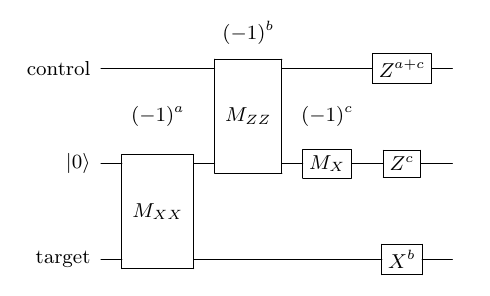
\includegraphics[scale=0.5]{img/cnotMeasureCircuit.png}\\
	\caption{A Quantum Circuit to implement a measurement based\\
		Controlled-$X_{|\psi\rangle_{control}\rightarrow |\psi\rangle_{target}}$ Gate,
		where $|0\rangle$ is the +1 eigenstate in $\sigma_{z}$-basis.}
	\label{fig:circuit1}
	\end{center}
\end{figure}
\newpage

As can be seen explicitly calculated in the familiar Schroedinger 
picture in Appendix~\ref{sec:calc1}, the circuit from figure~\ref{fig:circuit1}
implements a CNOT-gate from the control qubit to the target qubit.

We will now analyze this circuit in the Heisenberg picture,
finding that it results in an equal output.

\subsection{Heisenberg Picture and stabilizer Formalism}
\subsubsection{Stabilizer Group}
We call an operator/gate S, to which the input state is an 
eigenvector ($S|\psi\rangle=|\psi\rangle$), a ``stabilizer'' of that input state. \\
The ``stabilizer group'' is a generating subset of the set
of such operators.

We write these stabilizers as tensor-products of pauli operators
$P \in P_{G}$,
where pauli operators are the operators on $\mathbb{F}_{2}$ such that:

$\forall P\in P_{G}, n\in \mathbb{N}: P^{2n}=\mathbb{I}$.

In the Heisenberg picture, stabilizers are tracked instead of
states. 
The stabilizer group $S_{G}$ is the group generated by
the set of stabilizers:
\begin{equation}
	S_{G} = \langle S_{0},..,S_{n}\rangle: S|\psi_{in}\rangle = 
	|\psi_{in}\rangle \forall S \in S_{G}
\end{equation}

So for the example in figure~\ref{fig:circuit1} it is the group
of operators to whom
$|\psi_{control}\rangle \otimes |0\rangle \otimes 
|\psi_{target}\rangle$ is an eigenstate, namely 
$\mathbb{I}\otimes Z \otimes \mathbb{I}$ (and trivially
$\mathbb{I}\otimes\mathbb{I}\otimes\mathbb{I}$, which we choose
to ignore as a stabilizer since any three-qubit state
is stabilized by it, and it can be generated by squaring any
pauli-constructed stabilizer).

The stabilizer group is always an abelian group and its elements 
 commute, since if:

\begin{equation}
	\label{abelian_stabilizers_equation}
	\forall A,B \in S: AB|\psi\rangle = BA|\psi\rangle = |\psi\rangle
	\Rightarrow [A,B]|\psi\rangle=0
\end{equation}

\subsubsection{Effect of Gates on stabilizers}
In order to determine the effect a Gate operation A has on a
stabilizer, consider the following:

If $S|\psi\rangle = |\psi\rangle$ then:
\begin{equation}
A|\psi\rangle = AS|\psi\rangle = AS\mathbb{I}|\psi\rangle
	= \underbrace{ASA^{\dagger}}_{=S'}A|\psi\rangle
\end{equation}
So we now know that the post-gate state is an Eigenstate of $S'$.

Therefore $S'_{G} = \langle AS_{0}A^{\dagger},...,AS_{n}A^{\dagger}\rangle$.
%This generator expression can be further reduced by taking out
%all $S' \in S'_{G}$ for which $\exists J' \in S'_{G}: \{S',J'\}=0$

\subsubsection{Effect of measurements on stabilizers}
A pauli measurement operator M can either commute with all stabilizer
operators, in which case M itself is a stabilizer already and the
measurement has no effect on the state, or anticommute with at
least one operator in $S_{G}$, since pauli operators as well as
their tensor-products can only commute or anti-commute with each
other.

In that case, to obtain the new stabilizers  $S'_{G}$, proceed
as follows:
\begin{itemize}
	\item Identify $S\in S_{G}: {S,M}=0$
	\item Remove S from $S_G$
	\item Add $M$ to $S_G$ 
	\item for $N \in S_G \cup\overline{X}\cup\overline{Z}:$
		if $\{N,M\}==0: N=SN$ 
\end{itemize}
where $\overline{X}$ and $\overline{Z}$ are the sets of 
logical Xs and Zs respectively.

\subsubsection{Circuit Analysis in Stabilizer formalism}
After a measurement M, an n qubit input state will always 
collapse into either the +1 or the -1 eigenstate of the 
measurement operator.

In the first case the acting measurement operator becomes 
$\mathbb{I}^{\otimes n}+M$, in the second it becomes
$\mathbb{I}^{\otimes n}-M$. Therefore, in the circuit shown in 
figure~\ref{fig:circuit1}, the measurements are:

\begin{align}
	P^{\pm}_{1} &= \frac{1}{2}\left(\mathbb{I}^{\otimes 3} \pm 
	\mathbb{I}\otimes X \otimes X\right) \\
	P^{\pm}_{2} & = \frac{1}{2} \left(\mathbb{I}^{\otimes 3} \pm
	X \otimes X \otimes \mathbb{I}\right) \\
	P^{\pm}_{3} &= \frac{1}{2} \left(\mathbb{I}^{\otimes 3} \pm
	\mathbb{I} \otimes X \otimes \mathbb{I}\right)
\end{align}

In the following stabilizers
will be written without the tensorproduct symbols, so in 
our case the stabilizer is initially: $S_{G}^{0}= \langle IZI \rangle$,
the logical $\overline{X}$ operator is XXX and the logical
$\overline{Z}$ operator is ZIZ.

After the first Measurement, the state is stabilized by 
IXX, since it collapses into an eigenstate of the measurement 
operator. Notably, if the measurement operator M anticommutes
with some element of the stabilizer S:% $P^{+}_{1}$ and
%$P^{-}_{1}$ have the same stabilizers, since:

\begin{equation}
	SP_{-}S^{\dagger} = \frac{1}{2}S\left( 
	\mathbb{I}^{\otimes 3} - M \right) S^{\dagger}
	= \frac{1}{2} \left( \mathbb{I}^{\otimes 3} + M \right)
	SS^{\dagger} = P_{+}
\end{equation}

So by applying an anticommuting previous stabilizer operator
after the measurement one can ensure that the state is in the
$P_{+}$ projected state $P_{+}|\psi_{init}\rangle$ (in short,
+1 and -1 eigenstates have the same stabilizers if we add 
conditional gates accordingly).

For the logical operators, if $\overline{X}$ or $\overline{Z}$
do not commute with the measurement operator, we know that their
product with another anticommuting operator from the previous
stabilizer must then commute with the measurement operator: 
$[S_{prev}\overline{X}M, MS_{prev}\overline{X}]=0$ (recall the
previous statement that all paulis and their tensorproducts must
either commute or anti-commute).

In our case, IZI and IXX anticommute,
so now the state is stabilized by $S^{1}_{G} = \langle IXX
\rangle$. Both initial logical operators commute with the first
measurement operator, so are left unchanged.

After the second measurement $M_{2}$=ZZI, since this
measurement anticommutes with the IXX stabilizer, the new 
stabilizers are: $S^{2}_{G}=\langle ZZI \rangle$. The logical 
$\overline{X}$ and $\overline{Z}$ operators are unaffected
, since they commute with the measurement operator.

After the third measurement $M_{3}$ =IXI, since this measurement
anticommutes with the stabilizer, the new stabilizers are:
$S^{3}_{G}= \langle IXI \rangle$. The logical $\overline{Z}$
operator anticommutes with the measurement, so is replaced by\\
$ \overline{Z_{3}} $=ZZI $\cdot$ ZIZ = IIZ\@. The logical 
$ \overline{X} $ is unaffected, since it commutes with the
measurement operator. 

The stabilizer for the control and target qubit are still
identity, and logical $\overline{Z}: ZIZ \rightarrow IIZ$.

Since CNOT takes: $Z\otimes Z \rightarrow I \otimes Z$, this 
implements a logical CNOT.




